\begin{enumerate}[label=\thesubsection.\arabic*.,ref=\thesubsection.\theenumi]
\numberwithin{equation}{enumi}

\item Find the closed loop transfer function for the system in Fig. \label{fig:ee18btech11035_block} given that
\begin{align}
\label{eq:ee18btech11035_G(s)}
G\brak{s}=\frac{1}{s^2+2s}
\end{align}
%
\begin{figure}[!ht]
    \begin{center}
		\resizebox{\columnwidth}{!}{\tikzset{
        block/.style = {draw, rectangle,
            minimum height=1cm,
            minimum width=2cm},
        input/.style = {coordinate,node distance=1cm},
        output/.style = {coordinate,node distance=4cm},
        arrow/.style={draw, -latex,node distance=2cm},
        pinstyle/.style = {pin edge={latex-, black,node distance=2cm}},
        sum/.style = {draw, circle, node distance=1cm},
}

\begin{tikzpicture}[node distance=2.5cm,auto,>=latex']
  \node [input, name=input] {};
  \node [sum, right of=input] (sum) {};
  \node [block, right of = sum] (block1) {$k$};
  \node [block, right of = block1] (block2) {$G(s)$};
  \node [output, right of= block2] (output) {};
  \draw [->] (input) -- node {$r$} (sum);
  \draw [->] (sum) -- node {} (block1);
  \draw [->] (block1) -- node {} (block2);
  \draw [->] (block2) -- node [name =y] {$y$} (output);
  \draw [->] (y) -- ++ (0,-2) -| node [pos=0.99] {$-$} (sum);
\end{tikzpicture}}
	\end{center}
\caption{}
\label{fig:ee18btech11035_block}
\end{figure}
\\
\solution The closed loop transfer function is
\begin{align}
H\brak{s} &= \frac{kG\brak{s}}{1+kG\brak{s}}
\label{eq:ee18btech11035_4}
\\
 &= \frac{k}{s^2+2s+k}
\label{eq:ee18btech11035_H(s)}
\end{align}
after substituting from \eqref{eq:ee18btech11035_G(s)}.
\item Find the step response of the system.\\
\solution 
%The characteristics of the poles of transfer function describes the property of the transfer function.\\
%Calculating poles :
%\begin{align}
%    s^2+2s+k&=0\\
%    s&=\frac{-2\pm\sqrt{\brak{-2}^2-4\brak{1}\brak{k}}}{2\brak{1}}\\
%    \label{ee18btech11035_poles}
%    s&=-1\pm\sqrt{1-k}
%\end{align}
%
From \eqref{eq:ee18btech11035_H(s)}, the step response is 
%Calculating step response for a general damping system \eqref{eq:ee18btech11035_H(s)} :\\
\begin{align}
%X\brak{s}&=\frac{1}{s}\\
Y\brak{s}
%&=H\brak{s}X\brak{s}\\
&=\frac{k}{s^2+2s+k}\frac{1}{s}
\label{eq:ee18btech11035_ys}
\end{align}
\begin{multline}
\implies      y(t) = \lsbrak{1}
\\ +
\frac{k}{\brak{2\sqrt{1-k}}\brak{-1+\sqrt{1-k}}}{e^{\brak{-1+\sqrt{1-k}}}t}
\\
\rsbrak{+\frac{k}{\brak{2\sqrt{1-k}}\brak{1+\sqrt{1-k}}}{e^{\brak{-1-\sqrt{1-k}}}t}}u\brak{t}
\\
k \ne 1
\label{eq:y(t)}
\end{multline}
and
\begin{align}
y\brak{t}&=\brak{1-e^{-t}-te^{-t}}u\brak{t} \quad k=1
\end{align}
%
\item Find the steady state step response of the system usng the final value theorem.
\\
\solution From \eqref{eq:ee18btech11035_ys},
%
\begin{align}
\lim_{t\to\infty} y(t)&=\lim_{s\to0} sY(s)\\
&=1
\end{align}
\item Find the step response for an overdamped system.
\\
\solution For an overdamped system, $k < 1$,
\begin{multline}
\implies         y\brak{t} = \lsbrak{1 - e^{-t}\lcbrak{\frac{\sinh{\brak{\sqrt{1-k}}t}}{{\sqrt{1-k}}}}}
\\
+ \rsbrak{\rcbrak{\cosh\brak{\sqrt{1-k}}t}}u\brak{t}
\end{multline}
\item Find the step response for an underdamped system.
\\
\solution In this case, $k > 1$.
%
\begin{multline}
\implies         y\brak{t} = \lsbrak{1 - e^{-t}\lcbrak{\frac{\sin{\brak{\sqrt{k-1}}t}}{{\sqrt{k-1}}}}}
\\
+ \rsbrak{\rcbrak{\cos\brak{\sqrt{k-1}}t}}u\brak{t}
\end{multline}
\item Find the step response for a critically damped system.
\\
\solution For $k=1$,
\begin{align}
y\brak{t}&=\brak{1-e^{-t}-te^{-t}}u\brak{t}    
\end{align}


\item  The settling time $t_s$ is defined as the first instant where
%
\begin{align}
\abs{y(t_s)-y_{ss}} \le 0.02
\end{align}
where $y_{ss}$ is the steady state value of $y(t)$.  Find $k$ for which the settling time is minimum.
%Supposed the settling time is defined suto be the time taken to reach Find the settling time in terms of 'k' .\\
%\solution 
%\begin{align}
%0.98<y\brak{t}<1.02    
%\end{align}
%\begin{multline}
%\implies   0.98< 1\\ +\frac{k}{\brak{2\sqrt{1-k}}\brak{-1+\sqrt{1-k}}}{e^{\brak{-1+\sqrt{1-k}}}t} 
%\\
%+\frac{k}{\brak{2\sqrt{1-k}}\brak{1+\sqrt{1-k}}}{e^{\brak{-1-\sqrt{1-k}}}t}u\brak{t} < 1.02 \\
%\sbrak{\text{when }k\ne1}
%\label{eq:time}
%\end{multline}
%
%On further simplifying \eqref{eq:time}
%\begin{multline}
%\implies          -0.02 < \lsbrak{- e^{-t}\lcbrak{\frac{\sinh{\brak{\sqrt{1-k}}t}}{{\sqrt{1-k}}}}}
%\\
%+ \rsbrak{\rcbrak{\cosh\brak{\sqrt{1-k}}t}}u\brak{t} < 0.02
%\end{multline}

\solution Considering Critical Damped System,where $k=1$,\\
Plot of step response:
\begin{figure}[!h]
  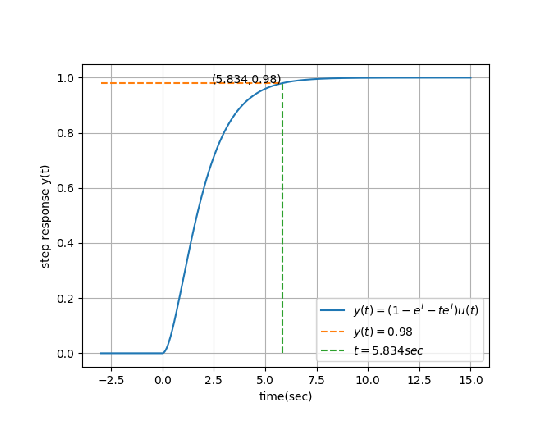
\includegraphics[width=\columnwidth]{./figures/ee18btech11035_1.eps}
  \caption{Step response of Critical damped system}
  \label{fig:ee18btech11035_1}
\end{figure}

Python code for above plot is
\begin{lstlisting}
codes/ee18btech11035_1.py
\end{lstlisting}

Settling time is 5.834sec.\\
Considering Under Damped System,where $k>1$
Plot of step response :
\begin{figure}[!h]
  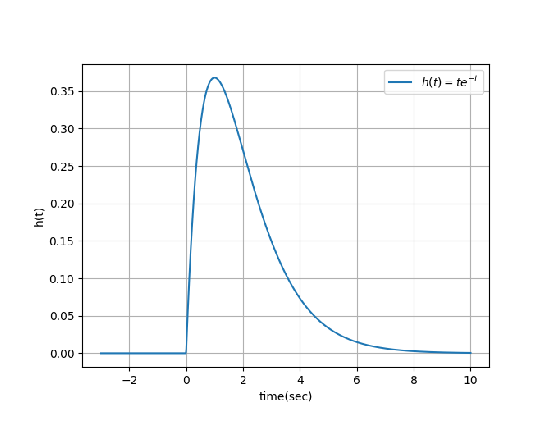
\includegraphics[width=\columnwidth]{./figures/ee18btech11035_2.eps}
  \caption{Step response of Under damped system}
  \label{fig:ee18btech11035_2}
\end{figure}

Python code for above plot is
\begin{lstlisting}
codes/ee18btech11035_2.py
\end{lstlisting}

There is an overshoot for every value of $k>1$.\\
Considering Over Damped System,where $k<1$\\
Plot of step response :
\begin{figure}[!h]
  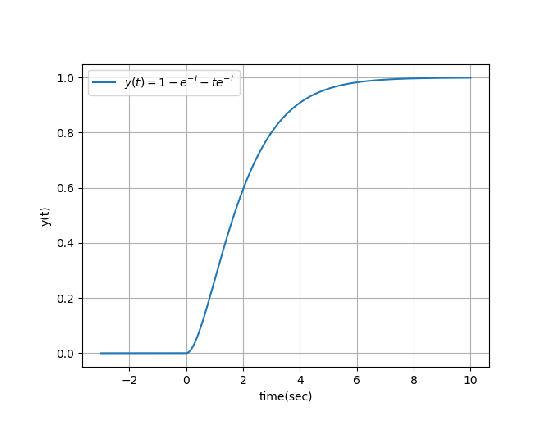
\includegraphics[width=\columnwidth]{./figures/ee18btech11035_3.eps}
  \caption{Step response of Over damped system}
  \label{fig:ee18btech11035_3}
\end{figure}

Python code for above plot is
\begin{lstlisting}
codes/ee18btech11035_3.py
\end{lstlisting}
As the value of $k$ is increasing the settling time is increasing.The lowest settling time obtained for a Over
damped system is greater than obtained for critical damped case.\\
Therefore, when $k$ is 1 minimum settling time for step response of the given system \eqref{eq:ee18btech11035_H(s)} is obtained.
\end{enumerate}
